\chapter{Giới thiệu}
\label{Chapter1}
\graphicspath{{Chapter1/Chapter1Figs}}

% Ngôn ngữ để viết và trình bày báo cáo khóa luận tốt nghiệp, đồ án tốt nghiệp, thực tập tốt nghiệp (sau đây gọi chung là báo cáo) là tiếng Việt hoặc tiếng Anh. 
% Trường hợp chọn ngôn ngữ tiếng Anh để viết và trình bày báo cáo,  sinh viên cần có đơn đề nghị, được cán bộ hướng dẫn (CBHD) đồng ý và nộp cho bộ phận Giáo vụ của Khoa vào thời điểm đăng ký đề tài để xin ý kiến.
% Báo cáo viết và trình bày bằng tiếng Anh phải có bản tóm tắt viết bằng tiếng Việt.


%Tóm tắt luận văn được trình bày nhiều nhất trong 24 trang in trên hai mặt giấy, cỡ chữ Times New Roman 11 của hệ soạn thảo Winword hoặc phần mềm soạn thảo Latex đối với các chuyên ngành thuộc ngành Toán.

%Mật độ chữ bình thường, không được nén hoặc kéo dãn khoảng cách giữa các chữ.
%Chế độ dãn dòng là Exactly 17pt.
%Lề trên, lề dưới, lề trái, lề phải đều là 1.5 cm.
%Các bảng biểu trình bày theo chiều ngang khổ giấy thì đầu bảng là lề trái của trang.
%Tóm tắt luận án phải phản ảnh trung thực kết cấu, bố cục và nội dung của luận án, phải ghi đầy đủ toàn văn kết luận của luận án.
%Mẫu trình bày trang bìa của tóm tắt luận văn (phụ lục 1).

% Với việc bùng nổ dữ liệu trên mạng Internet hiện nay, con người khó có thể nắm bắt được hết tất cả các thông tin.
% Do đó việc tìm kiếm dữ liệu, thông tin phù hợp với nhu cầu của bản thân dần trở nên khó khăn.
% Việc có một hệ thống gợi ý hỗ trợ chúng ta trong việc tìm kiếm thông tin là cực kỳ hữu ích. 
% Một hệ thống gợi ý sản phẩm là một bài toán trong lĩnh vực khai thác dữ liệu và học máy. 
% Hệ thống gợi ý được xây dựng để dự đoán những sản phẩm phù hợp với người dùng, đặc biệt hiện nay 
% việc đưa ra quyết định khi mà có quá nhiều lựa chọn dành cho người dùng là không hề dễ dàng. 
% Điều này dẫn đến vai trò của một hệ thống gợi ý ngày càng quan trọng hơn, 
% không chỉ hỗ trợ người dùng đưa ra quyết định mà còn đóng góp trong việc phát triển doanh nghiệp
%  khi mà việc thu hút khách hàng và nâng cao trải nghiệm người dùng sẽ phù thuộc vào 
% một hệ thống gợi ý sản phẩm hiệu quả. 
% Có rất nhiều lĩnh vực cần xây dựng hệ thống gợi ý có thể kể đến như thương mại điện thử, 
% các nền tàng cung cấp các dịch vụ đa phương tiện (âm thanh, hình ảnh, video, ...), 
% mạng xã hội (Facebook, tweeter, linkedin, ... ).  
% Theo số liệu tổng hợp được thì 75\% phim được thuê trên Netflix - một nền tảng cung cấp video nổi tiếng hiện nay đến từ hệ thống gợi ý; 38\% lượt click từ người dùng GOOGLE cũng đến từ hệ thống gợi ý và Amazon - một nền tảng mua bán trực tuyến mà 35\% sản phẩm được bán thông qua hệ thống gợi ý sản phẩm. 

% Để xây dựng một hệ thống gợi ý sản phẩm ta có các hướng tiếp cận là 


% Một trong những hướng nghiên cứu đang được quan tâm rộng rãi trong lĩnh vực trí tuệ nhân tạo gần đây
% là tạo ra các thuật toán giúp máy tính có thể ``hiểu'' được sở thích của người dùng và gợi ý cho họ
% các nội dung có liên quan. 

Hiện nay, với việc bùng nổ dữ liệu trên mạng Internet, người dùng có cơ hội tiếp cận
nhiều hơn với đa dạng các sản phẩm trên nền tảng số, song song đó,
các nhà cung cấp dịch vụ trên đó cũng có cơ hội tiếp cận với người dùng nhiều hơn. % đó = nền tảng số = internet
Tuy nhiên, người dùng đang gặp nhiều khó khăn khi tìm kiếm những nội dung phù hợp với nhu cầu của họ khi có quá nhiều sự lựa chọn.
Từ khó khăn đó, hệ thống gợi ý được xây dựng để dự đoán cho người dùng những nội dung - hay còn gọi là sản phẩm phù hợp với họ.
Hơn nữa, nó còn đóng vai trò quan trọng trong sự phát triển của các nhà cung cấp dịch vụ - doanh nghiệp,
khi góp phần giúp nâng cao trải nghiệm người dùng cũng như tăng sự thu hút khách hàng. Theo số liệu tổng hợp được, 
38\% lượt click từ người dùng Google đến từ hệ thống gợi ý và 
Amazon - một nền tảng mua bán trực tuyến mà 35\% sản phẩm được bán thông qua hệ thống gợi ý sản phẩm.

Trong lĩnh vực khoa học máy tính, hệ thống gợi ý sản phẩm là một chủ đề 
đang được quan tâm và nghiên cứu từ cộng đồng nghiên cứu khoa học.
Bài toán xây dựng hệ thống gợi ý được phát biểu như sau:
\begin{itemize}
    \item Đầu vào là lịch sử tương tác của người dùng (user) với các sản phẩm (items). 
    (các sản phẩm có thể là: quảng cáo, bộ phim, bài hát, văn bản để đọc, ... tùy thuộc vào lĩnh vực cụ thể)
    \item Yêu cầu máy tính tự động đưa ra các item (không có trong lịch sử) được dự đoán là phù hợp với người dùng.
    Chúng tôi gọi sản phẩm phù hợp với người dùng là sản phẩm được người dùng ``thích''.
\end{itemize}

Tuy nhiên, việc xây dựng một hệ thống gợi ý sản phẩm một cách hiệu quả là không đơn giản.
Đầu tiên, không có một ``lời giải'' chung cho tất cả trường hợp,
mặc dù đa số các lĩnh vực hiện nay đều có thể áp dụng các hệ thống gợi ý, tuy nhiên không phải là tất cả,
ta cần xét đến nhiều yếu tố khác nhau, 
từ đó mới có thể lựa chọn được ``cách'' để xây dựng hệ thống gợi ý phù hợp. % ``cách'' == ``hướng tiếp cận''
Từ thực tế cho thấy, các lĩnh vực mà sản phẩm ``tiêu thụ'' và ``sản xuất'' nhanh như: phim, hình ảnh, âm nhạc, ... 
thì hệ thống gợi ý sẽ ít nhiều đóng vai trò quan trọng. 
Theo số liệu tổng hợp được, một nền tảng cung cấp video nổi tiếng hiện nay - Netflix,
75\% số bộ phim được thuê đến từ hệ thống gợi ý, chứng tỏ sự ảnh hưởng lớn của hệ thống gợi ý đối với lĩnh vực này. 
Mặt khác, hệ thống gợi ý tác động không nhiều đến các lĩnh vực cung cấp dịch vụ hay sản phẩm giá trị cao như:
thuê nhà, phương tiện giao thông, thiết bị điện tử, ... người dùng cần đánh giá thông qua nhiều yếu tố mới có thể quyết định được. 
Thứ hai, tùy thuộc vào nhu cầu của người sử dụng mới có thể lựa chọn ``cách'' mà hệ thống gợi ý hoạt động.
Việc gợi ý các sản phẩm phù hợp với người dùng dựa vào nhóm người dùng có sở thích tương tự với họ 
hay dựa trên tính liên quan đến các sản phẩm họ đã ``thích'' trước đó là khác nhau. 
Điều này cũng liên quan đến khó khăn thứ ba khi xây dựng hệ thống gợi ý, cả trong cộng đồng nghiên cứu khoa học cũng như thực tiễn, 
ta cần một độ đo và một phương pháp để đánh giá một cách tổng thể và khách quan nhất, 
khi mà dữ liệu và các thuật toán để xây dựng hệ thống gợi ý là rất đa dạng.

Để xây dựng hệ thống gợi ý, một hướng tiếp cận chúng ta thường nghĩ ngay đến đầu tiên
là dự đoán các sản phẩm có ``độ tương đồng'' cao so với các sản phẩm người dùng đã ``thích'' trước đó,
hướng tiếp cận này được gọi là ``Content-Based Filtering'' (lọc dựa trên nội dung) (hình~\ref{fig_CBF} mô tả hướng tiếp cận này).
\begin{figure}
    \centering
	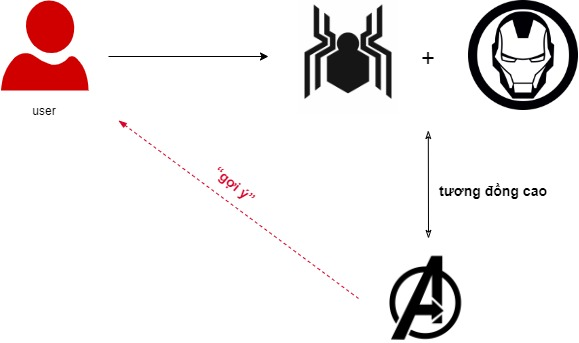
\includegraphics[width=0.6\textwidth]{CBF.jpg}
    \caption{Minh họa cách hoạt động của ``Content-Based Filtering'':
    mô hình gợi ý bộ phim có độ tương đồng cao với các bộ phim
    người dùng đã xem trước đó}
    \label{fig_CBF}
\end{figure}
Với hướng tiếp cận này, mô hình chỉ cần các thuộc tính mô tả của sản phẩm mà 
không đòi hỏi dữ liệu tương tác từ người dùng khác
vì các gợi ý là dành riêng cho từng cá nhân, do đó nó có khả năng nắm bắt tốt các sở thích
đặc biệt của người dùng.
Vì dựa trên tính tương đồng của sản phẩm, hệ thống có thể gợi ý cho người dùng một sản phẩm có ít sự quan tâm từ người dùng khác.
Để áp dụng ``Content-Based Filtering'' cho từng loại dữ liệu cụ thể,
ta cần ``domain knowledge'' cho lĩnh vực đó để thiết kế mô hình.
Trong trường hợp dữ liệu có ít mô tả chi tiết, hướng tiếp cận này vẫn còn hạn chế.

Một hướng tiếp cận khác là tìm ra ``độ tương đồng'' giữa các người dùng với nhau, hay tìm ra được một nhóm người dùng
có cùng sở thích dựa trên dữ liệu tương tác của tất cả người dùng. Khi đó, để có thể gợi ý cho một người dùng cụ thể,
hệ thống sẽ tìm các sản phẩm không có trong lịch sử của người dùng đó, và đã được những người dùng ``tương đồng'' tương tác,
hướng tiếp cận này gọi là ``Collaborative Filtering'' (lọc cộng tác) (hình~\ref{fig_CF} mô tả hướng tiếp cận này).
\begin{figure}
    \centering
    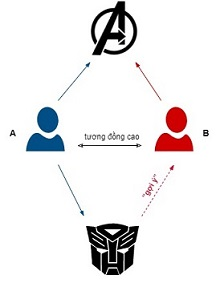
\includegraphics[width=0.4\textwidth]{CF.jpg}
    \caption{Minh họa cách hoạt động của ``Collaborative Filtering'': hai người dùng cùng xem một (hoặc nhiều) bộ phim 
    sẽ được hệ thống đánh giá là hai người dùng ``tương đồng'' nhau, khi đó một bộ phim được
    người dùng A xem sẽ được gợi ý cho người dùng B}
    \label{fig_CF}
\end{figure}
Đối với hướng tiếp cận ``Collaborative Filtering'', mô hình dựa vào lịch sử tương tác từ người dùng khác
và không cần các thuộc tính mô tả của sản phẩm, do đó nó có khả năng tạo ra sự tình cờ cho người dùng:
hệ thống có thể gợi ý một sản phẩm ``tốt'' cho người dùng trong trường hợp sản phẩm đó có ít điểm tương đồng
so với các sản phẩm người dùng đã ``thích'' trước đó. Dữ liệu đầu vào của hướng tiếp cận này là ma trận tương tác
của người dùng và sản phẩm, do đó có thể áp dụng cho nhiều lĩnh vực khác nhau mà không cần thiết kế lại hệ thống.
Tuy nhiên, ``Collaborative Filtering'' có một vấn đề tồn tại là vấn đề khởi động nguội (``cold-start''),
khi một người dùng mới đến với hệ thống thì hệ thống sẽ thường khó đưa ra được gợi ý tốt cho họ,
cũng như khi một sản phẩm được ít người dùng tương tác, hệ thống thường có xu hướng không gợi ý sản phẩm đó.

Ngoài ra, một hướng tiếp cận khác là ``Hybrid'', là sự kết hợp giữa hai hướng tiếp cận bên trên.
Trong luận văn này, chúng tôi chỉ tập trung tìm hiểu về hướng tiếp cận ``Collaborative Filtering''
vì hai lý do chính là ``Collaborative Filtering'' tổng quan hơn so với ``Content-Based Filtering''
- hướng tiếp cận cần ``domain knowledge'' cụ thể để thiết kế hệ thống cho từng lĩnh vực cụ thể
và với số lượng lớn cùng sự đa dạng của dữ liệu hiện nay,
ta quan tâm đến sở thích của người dùng nhiều hơn là độ tương đồng giữa các sản phẩm.

Một phương pháp để cài đặt cho ``Collaborative Filtering'' là sử dụng 
mô hình nhân tố ẩn (``latent factor model'') được Yu giới thiệu vào năm 2008, 







